% Appendix 6: The Occurrence of Reverse Perspective When Viewing Objects in Foreshortening
% Source pages: 262–270

\chapter{The Occurrence of Reverse Perspective When Viewing Objects in Foreshortening}

\srcpage{262}

The considerations presented in the preceding Appendix testify to the possibility of genuine
vision according to the laws of reverse perspective, provided that visual perception exhibits
``superconstancy''.  The weakness of that argument lies in the fact that, according to
current experimental data, the phenomenon of ``superconstancy'' is not registered in all
people.  Mathematical analysis shows, however, that the requirement of ``superconstancy''
is not necessary.  A person whose visual perception is characterised by only full---and even
somewhat incomplete---constancy can also see in reverse perspective (the discussion, as in
the preceding Appendix, concerns only distances of the order of a few metres).  This type
of visual perception is characteristic of the vast majority of people, not only under
binocular but also under monocular vision.

The mentioned effect will be observed in those cases when the parallel strips that a person
is looking at run not directly \emph{away from} the viewer, but at a slight \emph{angle}.

To take the decisive step in the analysis, it is necessary to introduce a highly important
concept---the \emph{zero line}.  Note the well-known inequality of the ``stretchings'' of
the retinal image by the visual-perception system in the $x$ and $y$ directions.  Recall
that the region of clear vision in man is comparatively small, and in surveying the space
before him a person involuntarily shifts his gaze from one region to another.  The region
on which he is looking at a given moment then serves as a kind of ``origin'', while all
other regions of space are assessed relative to it---they may be ``closer'', ``farther'',
``to the left'', ``to the right''.  The concepts ``closer'' and ``farther'' are, in a
certain sense, absolute, while ``to the left'' and ``to the right'' are relative: their
meaning does not change under turns of the head, whereas the concepts ``left'' and
``right'' can change their meaning under such turns.

Turning to an analytical treatment, we adopt the following notation.  Coordinates
$(\bar{x}_H, l)$ correspond to the subject plane, $(x_1, y_1)$ to the linear-perspective
system, and $(x_2, y_2)$ to the perceptual-perspective system.  The absence of subscripts
on $x$ and $y$ indicates that the statements made apply equally to two or all three of the
coordinate systems.

\srcpage{263}

The size-constancy mechanism will therefore always ``stretch'' the retinal image in the
$y$-direction uniformly, regardless of where the person looks (since this axis represents
movement ``near''---``far''), with the stretchings described by relation~(2.6).  As for
the stretchings along the $x$-axis, formula~(2.1) applies, linking $x_2$ not only
with~$l$ but also with~$x_1$---the distance of the point from some axis conventionally
taken as zero.  Movement parallel to the $x$-axis represents lateral movement.

In the previous Appendices it was always assumed that the person looks straight ahead,
perpendicular to the picture plane, and that the axis of the ``path'' runs in the same
direction.  In that case the image of the axis coincided with the principal axis of the
picture, which was naturally taken as the zero line from which the distances~$x_1$ were
measured left and right.  In passing to perceptual perspective, $x_1$ was multiplied
by~$P_1(l)$ to find~$x_2$.  Only points with $x_1 = 0$ underwent no lateral shifts,
since their new abscissa $x_2 = x_1 = 0$.

We define the \textbf{zero line} as the line that undergoes no lateral shifts in the
transition from the linear-perspective system to the perceptual-perspective system.

\begin{figure}[H]
    \centering
    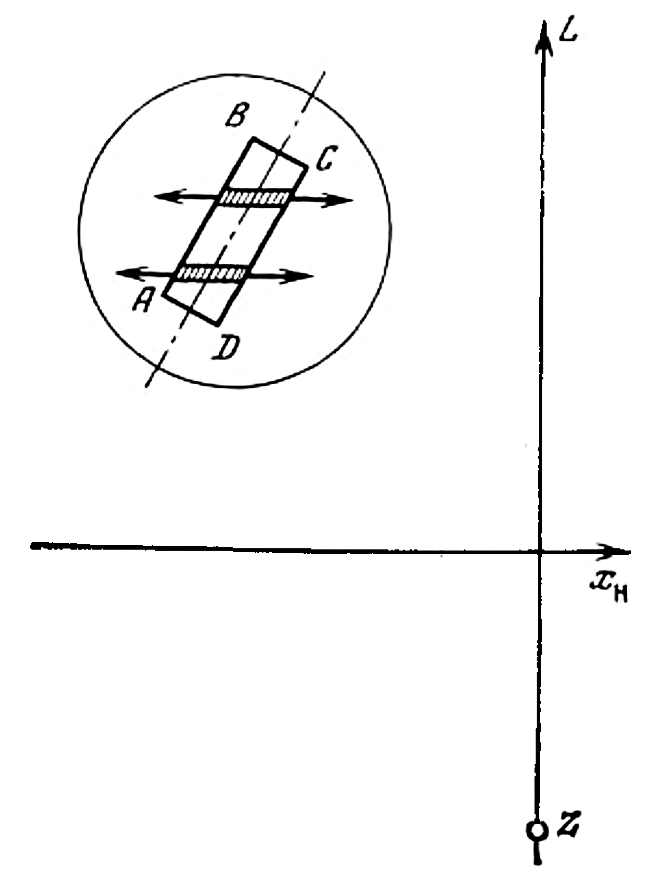
\includegraphics[width=0.4\linewidth]{figures/f6.1.png}
\end{figure}
\figblock{6.1}{Diagram of the subject plane (view from above) showing a viewer at point~1
  and a rectangle~$ABCD$ lying to one side of the depth axis.  The circle marks the region
  of clear vision.  Arrows indicate lateral ``stretchings'' away from the zero line
  (dash-dot), which is the axis of the rectangle rather than the depth axis.}

\srcpage{264}

In those cases when the sole object lies to one side of the depth axis (Fig.\,6.1), the
zero line turns out to be not the $l$-axis but the axis of rectangle $ABCD$ (dash-dot
line).  The zero line is determined by the central part of the retinal region of clear
vision; the stretchings proceed from it ``outward''.  It is not perpendicular to the
picture base but is inclined at an angle depending on the position of $ABCD$ on the
subject plane.

\begin{figure}[H]
    \centering
    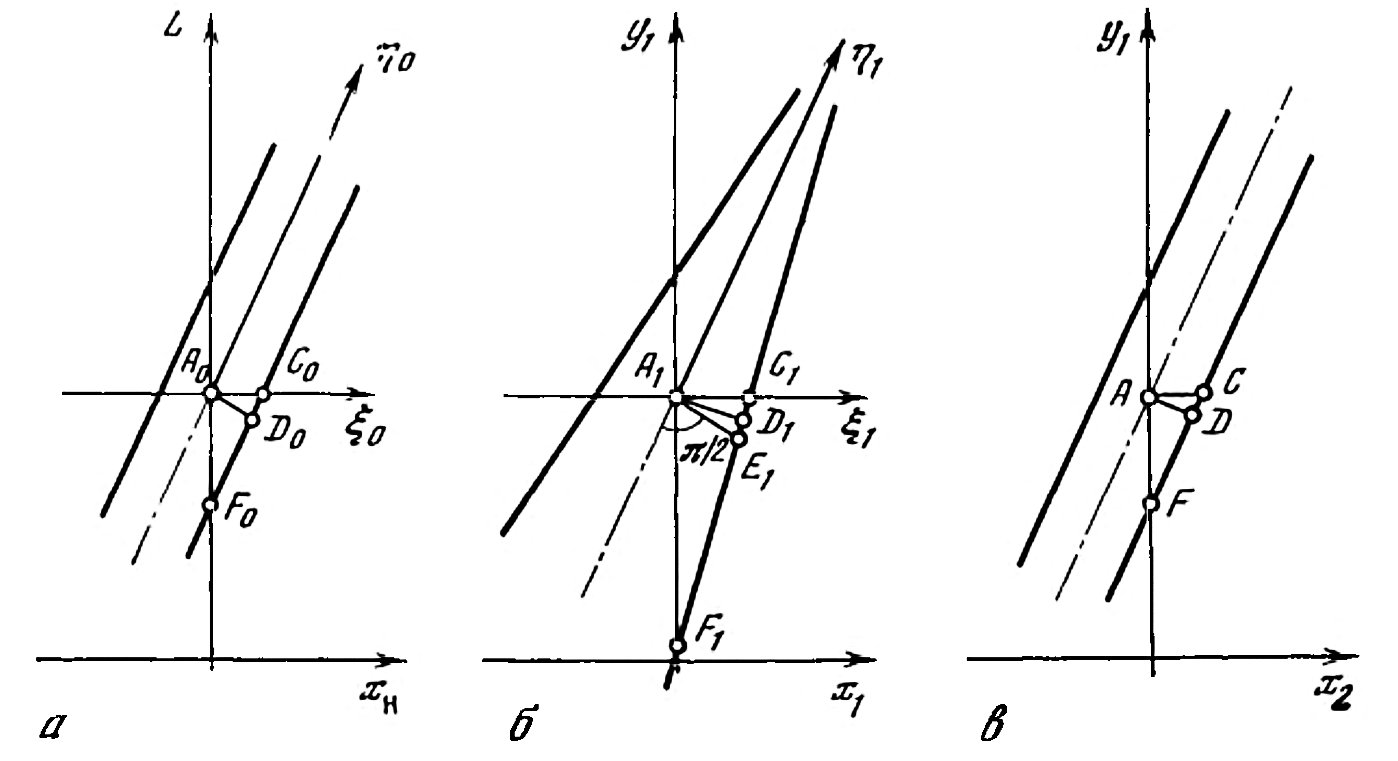
\includegraphics[width=1.0\linewidth]{figures/f6.2.png}
\end{figure}
\figblock{6.2}{Three-part scheme: (a)~subject plane with two parallel lines and the zero
  line; (b)~image in linear perspective; (c)~mixed coordinate image $(x_2, y_1)$
  showing the axis and near edge as parallel straight lines.}

For simplicity, we replace the elongated rectangle by a strip with parallel edges and
assume full constancy for near objects (not an obligatory assumption, as discussed below).
Our immediate aim is only the \emph{qualitative} proof that reverse-perspective perception
arises when contemplating a strip with parallel edges directed ``obliquely''.

Fig.\,6.2,\,a shows the subject plane (view from above) with two parallel lines [bars
over variable names indicate dimensionless notation according to formulas~(1.1)]:
\begin{align}
  \bar{l}^{**} &= \bar{a}_0'' + \bar{b}_0\,\bar{x}_H,  \tag{6.1a}\\
  \bar{l}^{*} &= \bar{a}_0' + \bar{b}_0\,\bar{x}_H.   \tag{6.1b}
\end{align}
($\bar{l}^{**}$ is the left, $\bar{l}^*$ the right line.)  We assume these lines to be
close together and that both pass (on the interval of~$\bar{x}_H$ under consideration)
near the picture plane, so that $l$ is small for all considered points.  The equation of
the axial line of the strip is
\begin{equation}
  \bar{l}_0^0 = \bar{a}_0^0 + b_0\,\bar{x}_H.  \tag{6.2}
\end{equation}
The smallness of~$l$ permits the assumption of full constancy, which requires choosing the
function $P_1$ in the form
\begin{equation}
  P_1(l) = 1 + l.  \tag{6.3}
\end{equation}

\srcpage{265}

Fig.\,6.2,\,b shows the image of the strip in linear perspective.  The equation of the
axial line in this system is
\begin{equation}
  y_1^0 = a_1^0 + b_1\,\hat{x}_1, \qquad
  a_1^0 = \frac{a_0^0}{1+a_0^0},\quad b_1 = \frac{b_0}{1+a_0^0}.  \tag{6.4}
\end{equation}

To describe the ``stretching'' of the retinal image using the zero-line concept, we
introduce an oblique coordinate system $(\xi_0, \eta_0)$ in the subject plane so that the
$\eta_0$-axis coincides with the zero line and the $\xi_0$-axis is parallel to~$\bar{x}_H$
(Fig.\,6.2,\,a).  The axial line has equation $\xi_0 = 0$ by definition, and the strip
edges have equations $\xi_0 = -c$ and $\xi_0 = c$, where $c$ is a constant.  On passing
to linear perspective, the oblique coordinate transforms as
\begin{equation}
  \xi_1 = \frac{\xi_0}{1 + l},  \tag{6.5}
\end{equation}
so that the right edge of the strip becomes
\begin{equation}
  \xi_1^* = \frac{c}{1+l}.  \tag{6.6}
\end{equation}

When the visual-perception system forms the perceptual space, $\xi_1^*$ is ``stretched''
[formula~(2.1)]: $\hat\xi_2^* = \xi_1^*\,P_1(l)$, whence, using~(6.3) and~(6.6),
\begin{equation}
  \hat\xi_2^* = \hat\xi_1^* P_1(l)  = c.  \tag{6.7}
\end{equation}

\srcpage{266}

We build the image of the strip in the auxiliary \emph{mixed} coordinate system $(x_2, y_1)$.
Since points of the zero line undergo no lateral shifts in passing from $(x_1, y_1)$ to
$(x_2, y_2)$, the equation of the zero line in the mixed system is the same as in
$(x_1, y_1)$:
\begin{equation}
  y_1^0 = a_1^0 + b_1\,\bar{x}_2.  \tag{6.8}
\end{equation}
For the near (lower in the schemes) edge, since $x_2 = x_1 + c$,
\begin{equation}
  y_1^* = a_1^* + b_1\,\bar{x}_2, \qquad a_1^* = a_1 - b_1\,c.  \tag{6.9}
\end{equation}
Comparing~(6.8) and~(6.9) shows that in the mixed system the axial line and the near edge
have become \emph{parallel} straight lines (see Fig.\,6.2,\,c).

To pass to the perceptual-perspective system one accounts for the $y$-direction stretching.
Since this stretching proceeds according to relation~(2.6), in which $x$-coordinates do
not appear, both lines transform identically:
\begin{equation}
  dy_2 = P_1(l)\,dy_1.  \tag{6.10}
\end{equation}
Using~(6.3) together with~(6.10) and equations~(6.8)--(6.9), one obtains
\begin{equation}
  \frac{dy_2^{\,\text{axis}}}{dx_2} = b_1(1+l_A),\qquad
  \frac{dy_2^{\,\text{near}}}{dx_2} = b_1(1+l_B).  \tag{6.11}
\end{equation}

These expressions determine the slopes of the tangent lines relative to the $x_2$-axis.
Since the $x$-coordinates do not appear in~(6.11), for simplicity consider the region near
the $y$-axis.  For all points lying below~$C_0$ on the near edge, the values of~$l$
are smaller than at point~$A_0$ on the axis (e.g.\ $l_B < l_A$), since the strips
are inclined with~$b_0 > 0$.  This gives the inequality

\srcpage{267}

\begin{equation}
  \left.\frac{dy_2^0}{dx_2}\right|_A > \left.\frac{dy_2^*}{dx_2}\right|_D,  \tag{6.12}
\end{equation}
which says that in perceptual space objectively parallel lines are seen as diverging with
increasing depth---the axial line appears steeper than the near edge.  \emph{This is the
reverse perspective.}  As is clear from the argument, the conclusion is unchanged if one
compares point~$A_0$ with~$E_0$, or with a point lying on the perpendicular to the
perceptual-perspective image of the axial line.

Consequently, when viewing near, narrow strips with objectively parallel edges arranged
``obliquely'', a person sees them in reverse perspective.  Thus reverse perspective is a
\emph{norm} of human vision at short distances.  The present considerations indicate a
method by which a modern person too can see space in reverse perspective; it is described
in Chapter~V.

\begin{figure}[H]
    \centering
    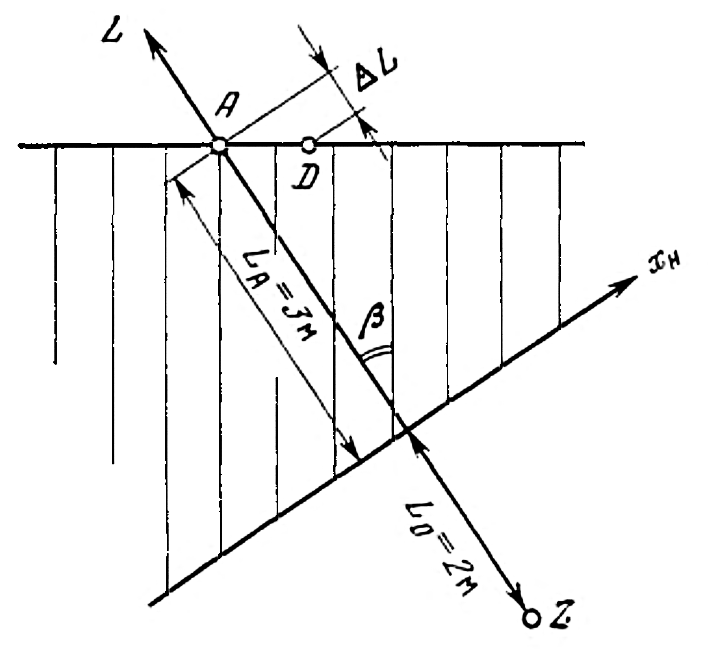
\includegraphics[width=0.6\linewidth]{figures/f6.3.png}
\end{figure}
\figblock{6.3}{Plan of a room with parquet strips of width~$B$.  The viewer stands at
  point~$I$ and looks in the direction making angle~$\beta$ with the strip structure.
  The far wall $AD$ is 5\,m away.}

Although the derivations above were intended to give only a qualitative proof, the
obtained expressions permit quantitative estimates.  Consider the example of observing the
parallel structure of a floor.  Fig.\,6.3 shows a plan of a room with parquet strips of
width~$B$; the viewer stands at point~$I$ and looks in a direction making angle~$\beta$
with the linear structure of the floor.  The far wall is 5\,m from the viewer.

\srcpage{268}

We estimate the angular divergence of a group of parallel parquet strips in the region of
the far wall.  The angle~$\beta$ is chosen to give the maximum divergence effect.

Using formulas~(1.1) and the results of the present Appendix,
\begin{equation}
  \frac{dy_2}{dx_2} = \frac{Hb_1(1+l/l_0)^2}{B},  \tag{6.13}
\end{equation}
where
\begin{equation}
  b_1 = \frac{b_0}{1+a_0},\quad a_0 = \frac{a}{b_0},\quad l_0 = \frac{bB}{l_0}.
  \tag{6.14}
\end{equation}
(It should be remembered that $b_1$ is computed at point~$A$.)

The angle of non-parallelism of the strip boundaries at points $A$ and $D$ in visual
perception is
\begin{equation}
  \alpha = \arctan\!\left.\frac{dy_2}{dx_2}\right|_A
         - \arctan\!\left.\frac{dy_2}{dx_2}\right|_D  \tag{}
\end{equation}
Assuming the depths of $A$ and $D$ to be close and writing $l_D = l_A - \Delta l$
($\Delta l$ small), one obtains the approximate formula
\begin{equation}
  \alpha = \frac{d}{dl}
         \arctan\!\left.\frac{dy_2}{dx_2}\right|_A \Delta l  \tag{6.15}
\end{equation}
\begin{equation}
  \alpha \approx \frac{\Delta l \ b_1\,H/Bl_0}
    {1 + \bigl[b_1\,H(1+l_A/l_0)/B\bigr]^2}.  \tag{6.16}
\end{equation}

Setting $d\alpha/db_1 = 0$ to maximise~$\alpha$ with respect to the direction of gaze,
\begin{equation}
  b_1^{\,*} = \frac{B}{H(1+l_A)};  \tag{6.17}
\end{equation}
here and below asterisks mark quantities giving the maximum of~$\alpha$.  The
corresponding optimal slope $b^*$ (determining the angle $\beta^*$ in Fig.\,6.3) is
\begin{equation}
  b^* = \frac{l_0}{H}.  \tag{6.18}
\end{equation}
Substituting~(6.17) into~(6.16):
\begin{equation}
  \alpha^* = \frac{\Delta l}{2(l_0 + l_A/l_0)}.  \tag{6.19}
\end{equation}

\srcpage{269}

Formulas~(6.18) and~(6.19) give the optimal direction of gaze and the expected angular
divergence of objectively parallel strips (in radians).

A noteworthy result is that both quantities are independent of~$B$.  In the present
example $b^* \approx 1.25$, i.e.\ $\beta^* \approx 39°$.  To compute~$\alpha^*$ one
must specify~$\Delta l$.  Following Fig.\,6.3, $\Delta l = AD\sin\beta^*$, showing the
natural growth of~$\alpha^*$ with increasing strip width.  Taking as a reasonable
value $\Delta H = 1.5$\,m fitting within the zone of clear vision, one immediately
obtains $\alpha^* \approx 6°$.  Thus the probable magnitude of the visible angular
divergence of objectively parallel strips amounts to several degrees and can hardly
exceed~$10°$.

\begin{figure}[H]
    \centering
    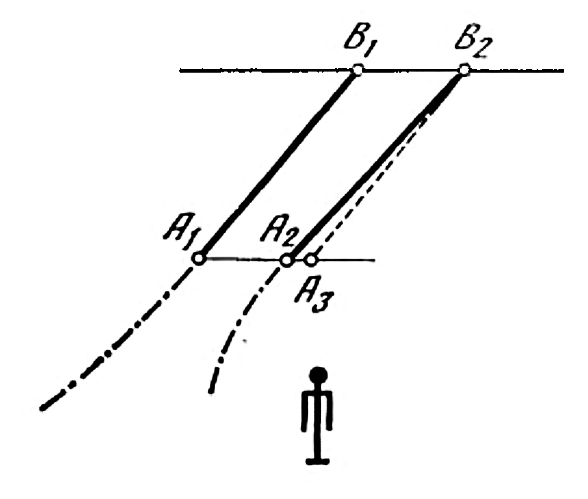
\includegraphics[width=0.45\linewidth]{figures/f6.4.png}
\end{figure}
\figblock{6.4}{Results of the author's experiments.  Objectively parallel lines viewed
  obliquely at $20°$--$30°$ and fixated at 4--6\,m appear to diverge from~$A_1A_2$ to
  the far wall~$B_1B_2$.  Closer to the observer the same lines appear to converge
  (dashed lines), since the peripheral visual field is aconstant.}

The numerical estimates obtained here agree well with the experimental data cited below,
and this is all the more remarkable since no experimental constants were employed in the
derivation.  In essence, both the qualitative and quantitative results rest on only two
assumptions: the hypothesis of the existence of a zero line, and the condition that at
short distances human vision is characterised by full constancy.

The last assumption can be substantially relaxed.  Since the resulting reverse perspective
is sufficiently large, it may be assumed that visual perception exhibits incomplete
constancy.  For example, if under full constancy reverse perspective amounts to about~$5°$,
and if due to incomplete constancy the observer perceives the parallel edges of a strip
seen along their length as slightly converging (with a convergence angle of~$3°$--$4°$),
it is not difficult to see that when looking at them ``obliquely'' he can perceive a weak
reverse perspective of~$1°$--$2°$.

\srcpage{270}

Let us examine some experimental data confirming the above propositions.

As far as the author is aware, the first to describe genuine vision in reverse perspective
was A.~Bakushinsky.\footnote{See: \emph{Iskusstvo}, 1923, No.\,1, p.\,235.}  Having
developed his own, somewhat erroneous, theory (see Ch.\,IV), he was psychologically
prepared to see objects in reverse perspective, and he actually did so.  Here is his
description: ``\ldots the perception of books of the same format and size, scattered on
the floor in depth from the viewer\ldots The impression will be as follows: the visible
rectangles, increasing in their sizes in reverse perspective up to a certain point in
depth, will thereafter diminish and foreshorten in normal perspective.''  Unfortunately,
Bakushinsky gave no numerical data connected with his observations, and his remark that
one can see city roofs in reverse perspective from a bell-tower arouses doubt (this is
probably an armchair conclusion).

The experiments carried out by the author consisted in observing clear and manifestly
parallel lines (edges of a carpet runner, parquet strips, large rectangular floor
patterns, etc.) by the method of Appendix~3 (see Fig.\,3.2).  The width of the
formations ranged from 0.5 to~1.2\,m and the depth from 5 to~8\,m.  Observations were
made indoors, sitting and standing.  The reverse-perspective effect was observed when
contemplating parallel lines ``receding'' from the viewer if they lay somewhat to one
side ($20°$--$30°$ in the described experiments) and when the gaze was fixed on a
section 4--6\,m from the viewer.  Objectively parallel lines appeared slightly diverging
(Fig.\,6.4), from a certain distance~$A_1A_2$ up to the far wall~$B_1B_2$.  Measurement
gave a point~$A_3$ to the right of~$A_2$ when a line parallel to~$A_1B_1$ was
constructed from~$B_2$ by the ruler method.  The distance~$A_2A_3$ amounted to
approximately 5--10\% of~$A_1A_2$, corresponding to a divergence angle of about
$2°$--$3°$.  When the gaze was fixed on the far part of the parallel lines, the near
section (closer than~$A_1A_2$) appeared to converge in depth---obeying normal
perspective (dash-dot lines in Fig.\,6.4).  This is connected with the aconstancy of
peripheral vision: in the peripheral visual field an image close to the retinal image
arises.
